% Created 2020-04-01 mié 08:59
% Intended LaTeX compiler: pdflatex
\documentclass[presentation,aspectratio=1610]{beamer}
\usepackage[utf8]{inputenc}
\usepackage[T1]{fontenc}
\usepackage{graphicx}
\usepackage{grffile}
\usepackage{longtable}
\usepackage{wrapfig}
\usepackage{rotating}
\usepackage[normalem]{ulem}
\usepackage{amsmath}
\usepackage{textcomp}
\usepackage{amssymb}
\usepackage{capt-of}
\usepackage{hyperref}
\usepackage{khpreamble}
\usepackage{pgfplots}
\usepackage{pdfpages}
\usepgfplotslibrary{groupplots}
\usetheme{default}
\author{Kjartan Halvorsen}
\date{\today}
\title{System identification of the pneumatic tank model}
\hypersetup{
 pdfauthor={Kjartan Halvorsen},
 pdftitle={System identification of the pneumatic tank model},
 pdfkeywords={},
 pdfsubject={},
 pdfcreator={Emacs 26.3 (Org mode 9.3.6)}, 
 pdflang={English}}
\begin{document}

\maketitle

\section{Intro}
\label{sec:org067222b}
\begin{frame}[label={sec:orge13f9f7}]{Lab experiment}
\begin{center}
\includegraphics[width=\linewidth]{../../figures/tank-lab-setup.png}
\end{center}
\end{frame}

\begin{frame}[label={sec:org9936e26}]{Simulink simulation}
\begin{center}
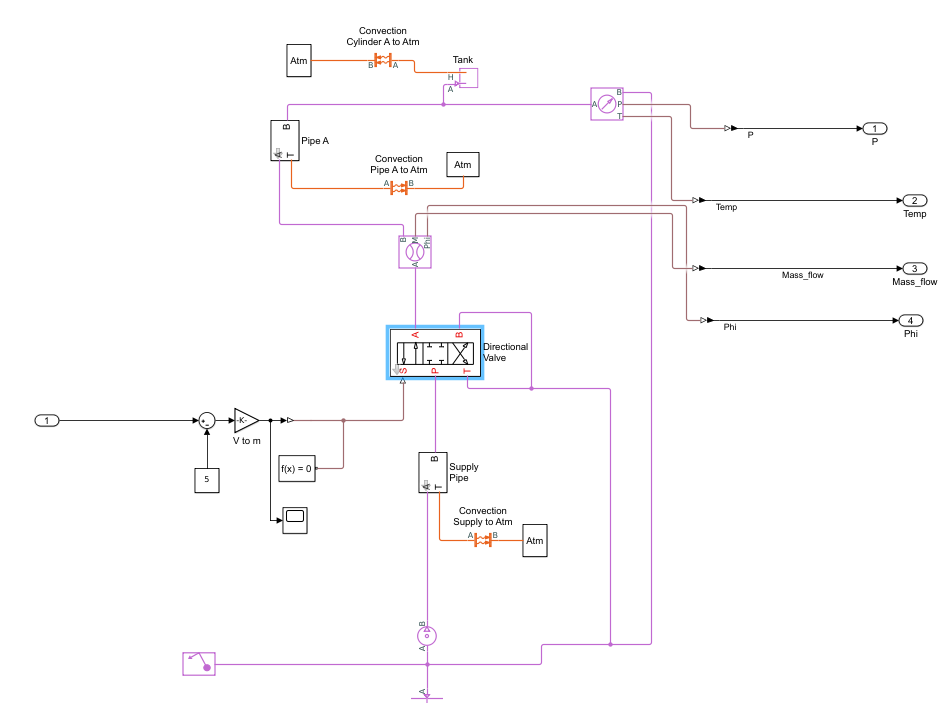
\includegraphics[width=0.8\linewidth]{../../figures/tank-simscape-model.png}
\end{center}
\end{frame}

\section{Models}
\label{sec:org432c17d}
\begin{frame}[label={sec:orgcb96d48}]{System identification}
\begin{center}
  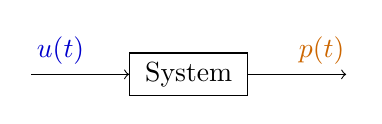
\begin{tikzpicture}[node distance=22mm, block/.style={rectangle, draw, minimum width=15mm}, sumnode/.style={circle, draw, inner sep=2pt}]

    \node[coordinate] (input) {};
    \node[block, right of=input, node distance=20mm] (plant)  {System};
    \node[coordinate, right of=plant, node distance=20mm] (output) {};

    \draw[->] (input) -- node[above, pos=0.3, color=blue!80!black] {$u(t)$} (plant);
    \draw[->] (plant) -- node[above, near end, color=orange!80!black] {$p(t)$} (output);
  \end{tikzpicture}
\end{center}   

Given input-output data \(\{ \big( \textcolor{blue!80!black}{u(1)}, \textcolor{orange!80!black}{p(1)} \big), \big( \textcolor{blue!80!black}{u(2)}, \textcolor{orange!80!black}{p(2)} \big), \ldots, \big( \textcolor{blue!80!black}{u(N)}, \textcolor{orange!80!black}{p(N)} \big) \}\) find a \alert{good description} of the system that generated the data.
\end{frame}

\begin{frame}[label={sec:org0d412e7}]{Flow through the valve}
\begin{center}
  \begin{tikzpicture}
    \node {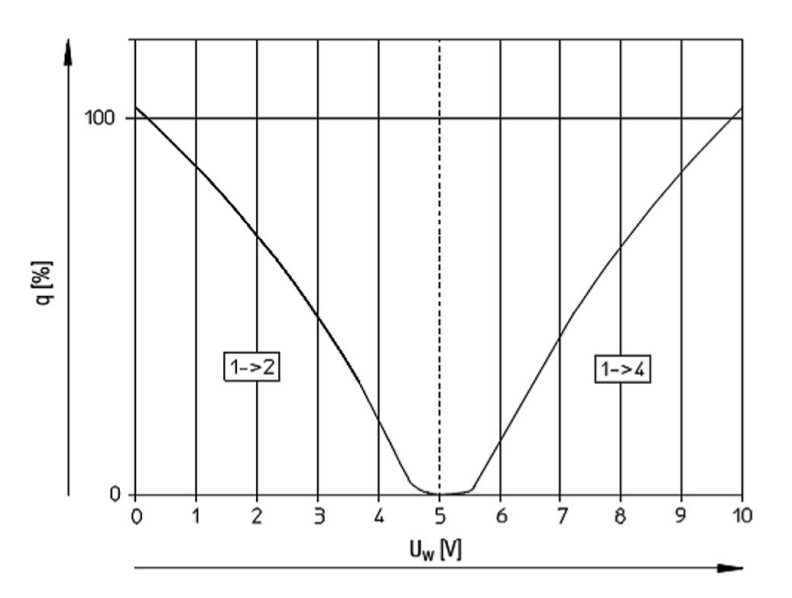
\includegraphics[width=0.7\linewidth]{../../figures/valve-volt-opening.png}};
    \node[coordinate] (five) at (0.54,-2.8) {};
    \node[coordinate, below of=five, node distance=1.8cm] (origin) {};
    \draw[color=red!80!black] (five) to (origin);
    \draw[color=blue!80!black, ->, thick] (origin) ++(0,0.4cm) -- node[below, near end] {$u(t)$} ++(1.5cm, 0); 
   \end{tikzpicture}
\end{center}
\end{frame}


\begin{frame}[label={sec:org2499e40}]{Nonlinear model 1}
\begin{block}{Flow into the tank, \(V_{in}(t) > 5\)}
\[ \dot{p}(t) = a_0(\underbrace{V_{in}(t) - 5}_{u(t)})\sqrt{|\underbrace{p_s - p(t)}_{\Delta p(t)}|} \]
\end{block}
\begin{block}{Flow out the tank, \(V_{in}(t) < 5\)}
\[ \dot{p}(t) = a_0u(t)\sqrt{|\underbrace{p(t)-0}_{\Delta p(t)}|} \]
\end{block}
\end{frame}

\begin{frame}[label={sec:orgc8a4915}]{Nonlinear model 2}
\[ \dot{p}(t) = a_0u(t)|\Delta p(t))|^{a_1} \]
\end{frame}

\begin{frame}[label={sec:org5ac1def}]{Converting to a regression model which is linear in the parameters}
\[ \dot{p}(t) = a_0u(t)|\Delta p(t)|^{a_1} \]

Take the logarithm of the equation to get

\[ \log \dot{p} = \log a_0 + \log u + a_1 \log |\Delta p|\]
\end{frame}

\begin{frame}[label={sec:org3d7146d}]{Linear model}
Introduce \(y(t) = p(t)-p_0\), where \(p_0\) is a chosen operating point.

\[ \dot{p}(t) = \dot{y}(t) = -a y(t) + ku(t)\]
\end{frame}


\section{Experiments and results}
\label{sec:orga687e3f}

\begin{frame}[label={sec:org687b35d}]{Input-output data}
\begin{center}
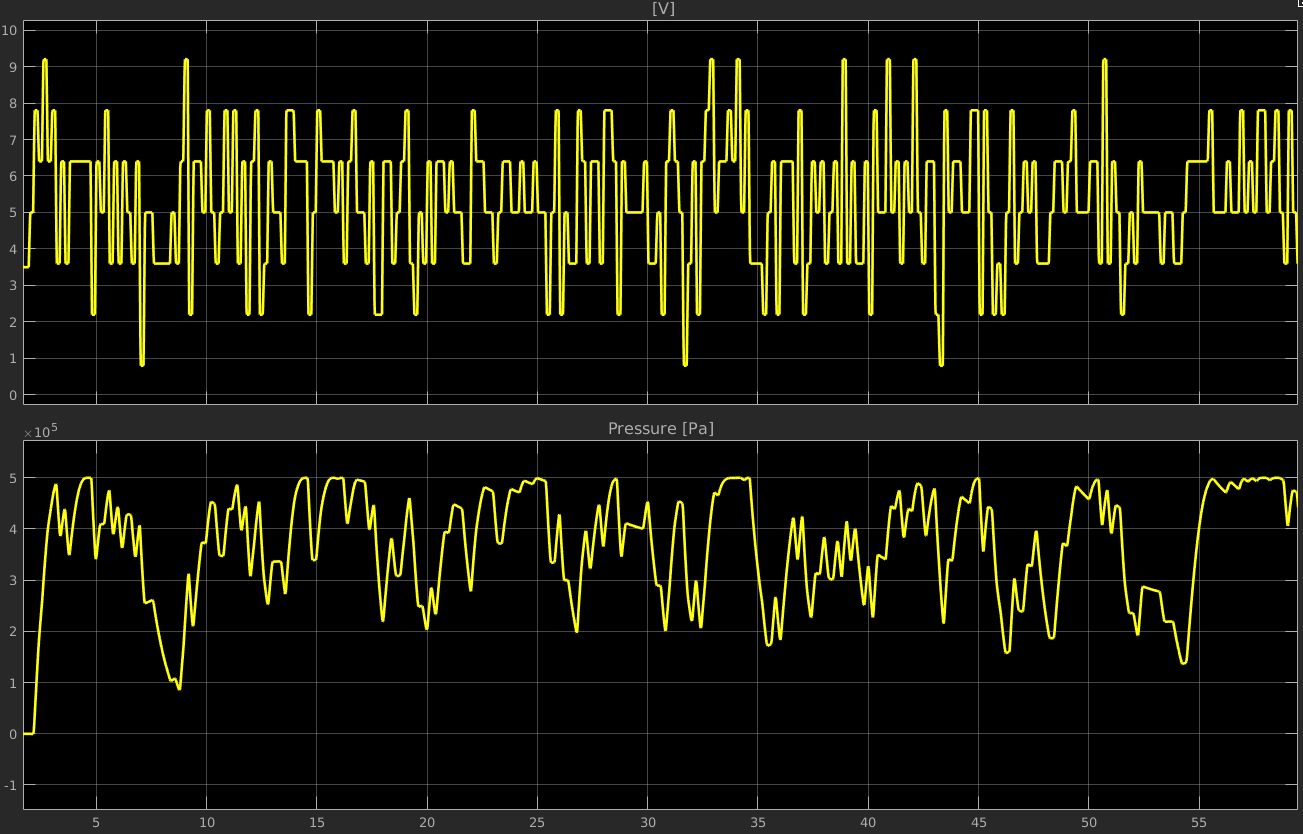
\includegraphics[width=0.88\linewidth]{../../figures/tank-sysid-input-output.png}
\end{center}
\end{frame}

\begin{frame}[label={sec:orgd55b88c}]{Fitting nonlinear model 1}
\begin{center}
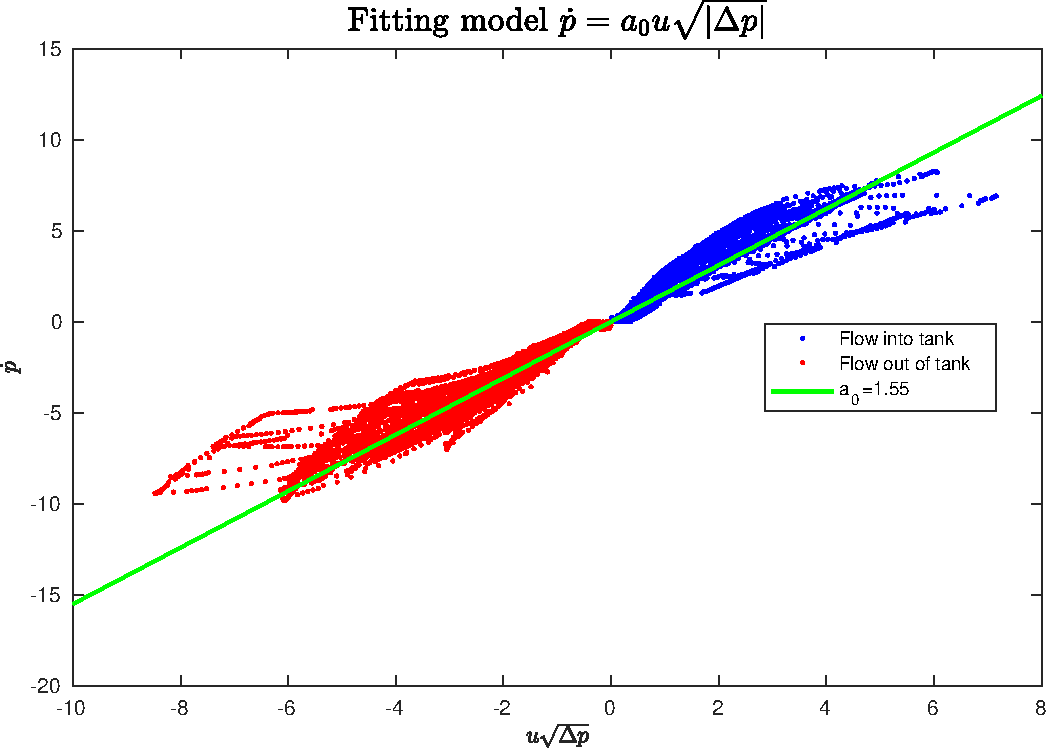
\includegraphics[width=0.9\linewidth]{../../figures/tank-sysid-sqrt-deltaP}
\end{center}
\end{frame}

\begin{frame}[label={sec:orgc3a7756}]{Fitting nonlinear model 2}
\begin{center}
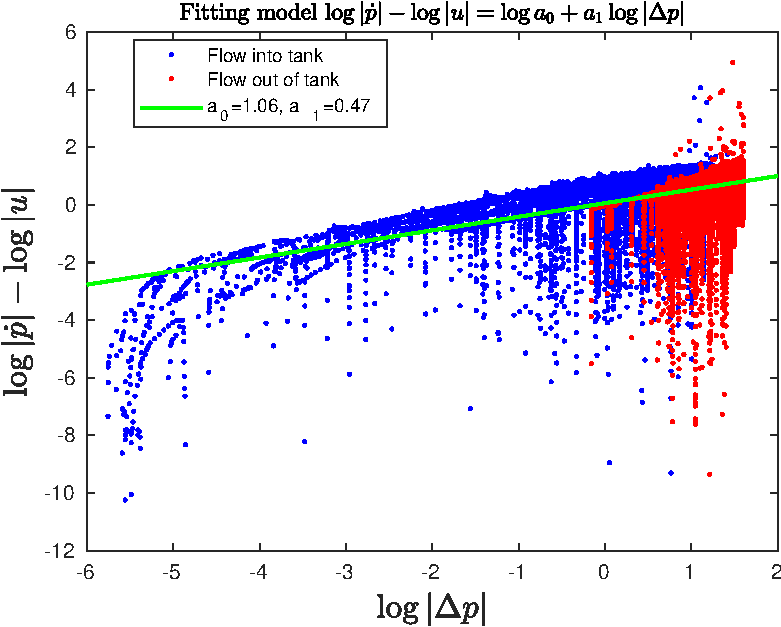
\includegraphics[width=0.8\linewidth]{../../figures/tank-sysid-log}
\end{center}
\end{frame}

\begin{frame}[label={sec:org54e1900}]{Fitting linear model}
\begin{center}
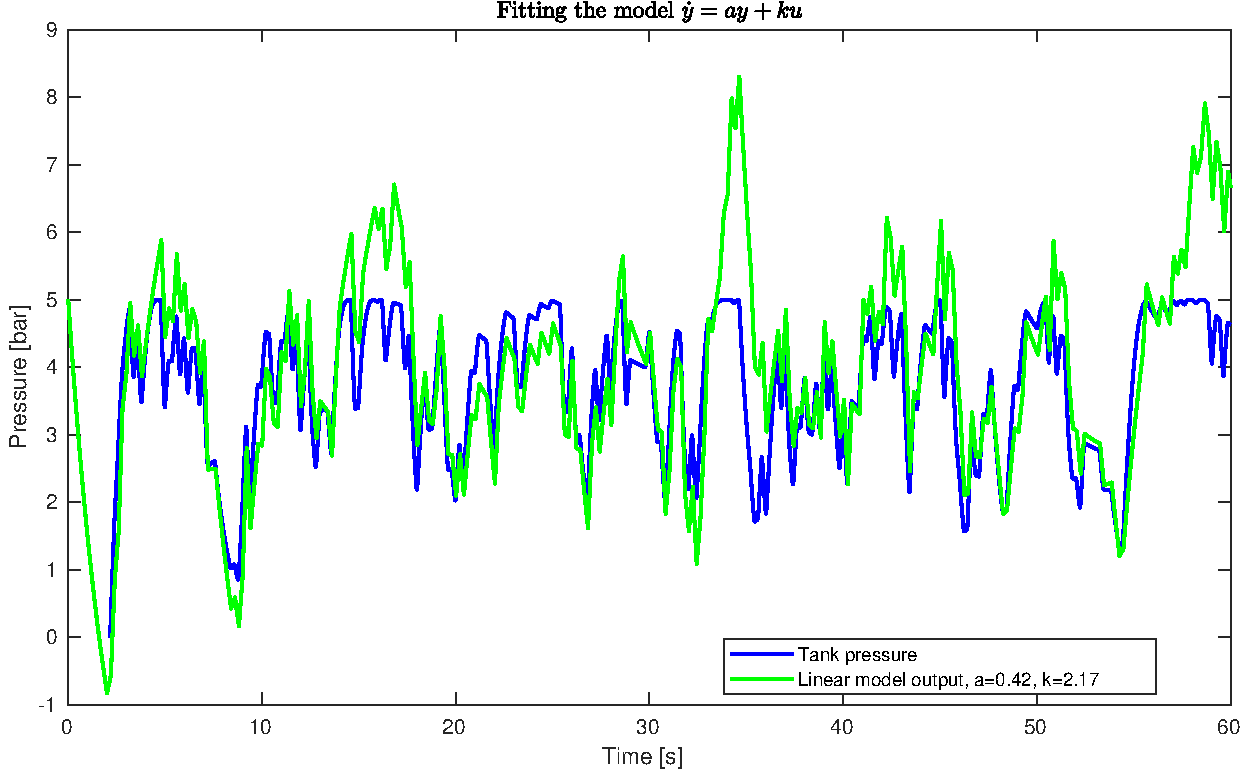
\includegraphics[width=0.8\linewidth]{../../figures/tank-sysid-linear-model}
\end{center}
\end{frame}

\begin{frame}[label={sec:org23ab816}]{Validation}
\begin{center}
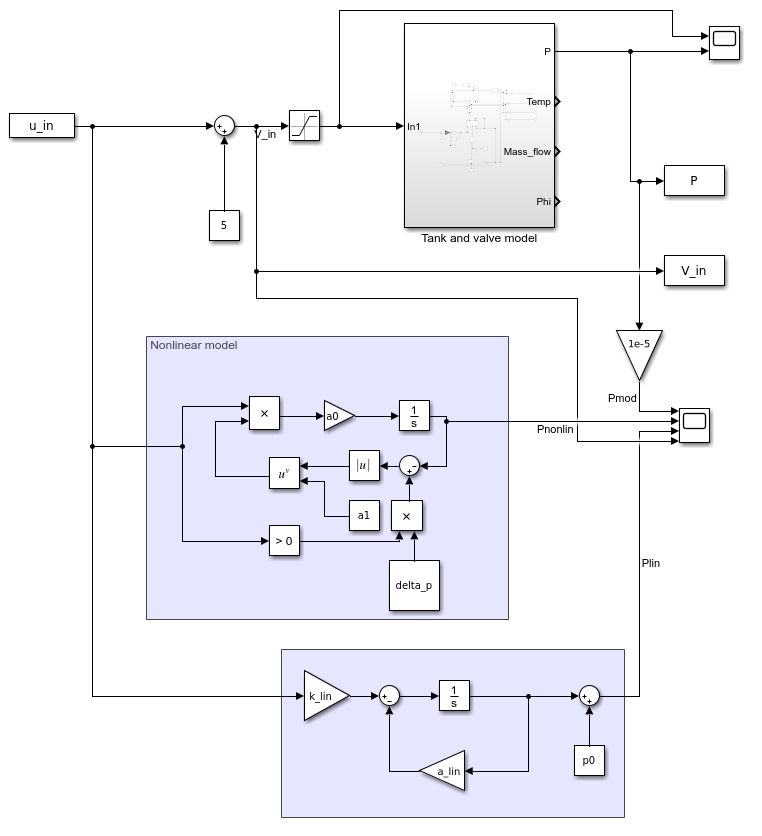
\includegraphics[width=0.55\linewidth]{../../figures/sysid-tank-validation-model.png}
\end{center}
\end{frame}

\begin{frame}[label={sec:orgc0ea29b}]{Validation results}
\begin{center}
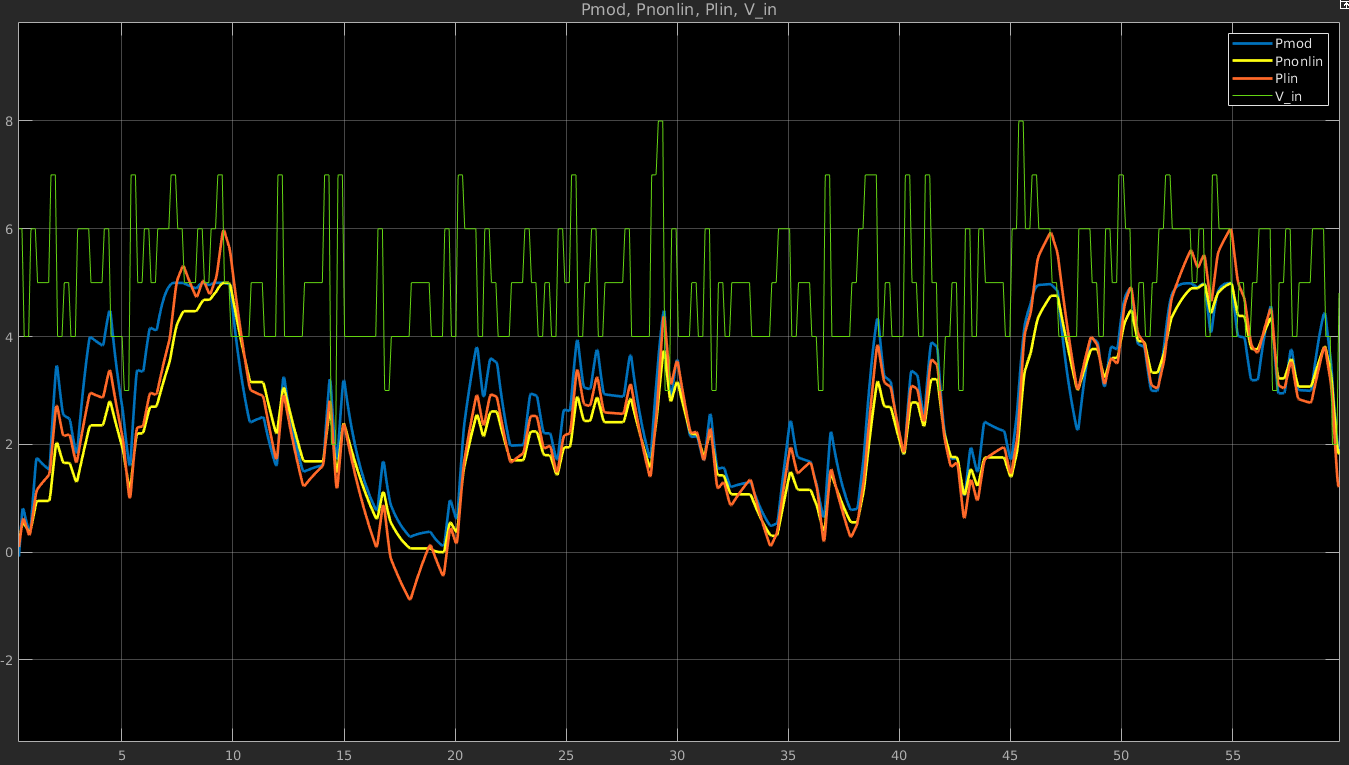
\includegraphics[width=\linewidth]{../../figures/sysid-tank-valudation-results.png}
\end{center}
\end{frame}
\end{document}